\section{Introduction}\label{sec:intro}
\vspace{-1pt}


\IEEEPARstart{T}{oday}, cloud providers (e.g., AWS~\cite{aws:region}, Azure~\cite{azure:region}, and Huawei~\cite{huawei:region}) host computing infrastructures across multiple global locations. These infrastructures are typically organized into regions, each strategically designed to offer computing services in proximity to clients. As a result, multi-region deployment has emerged as a prominent choice for cloud-native applications aiming for stringent client-perceived latency, high availability, strong scalability, and effective service localization~\cite{dast:eurosys21, ov:vldb19, taft2020cockroachdb, vanbenschoten2022enabling, zhang2018building}.

In pursuit of scalability and availability, these applications frequently partition and replicate their data storage across multiple servers (nodes). Each partition, known as a data shard, maintains a primary replica. The primary replica is consistently deployed in the region where the majority of access requests originate, ensuring optimal locality. \fig{fig:intro} provides an overview of our multi-region deployment model, which is fueled by the desire of global companies to not only build scalable applications but also control with fine granularity where data resides for good performance and meet the data governance policies (e.g., GDPR~\cite{GeneralD60:online}).



However, supporting serializable ACID transactions in such applications presents a perpetual challenge. Coordinating a cross-region transaction (CRT) is always slow due to geographic distances. For example, a cross-region transaction incurs a $\sim50ms$ network delay from Hong Kong to Singapore, whereas the network delay within a region is less than $2ms$ when powered by modern network technologies (e.g., dedicated inter-datacenter networks~\cite{aws:region}). 

Several impressive works (e.g., ~\cite{ov:vldb19, nguyen2023detock, slog:vldb19, calvin, janus:osdi16}) have been proposed to enhance the performance of geo-distributed transactions. These strategies involve redesigning critical aspects of concurrency control protocols or eliminating CRTs by making certain assumptions about the workloads. However, we emphasize that CRTs remain essential for general workloads, such as those with limited prior knowledge of application semantics or those employing interactive transactions. Moreover, the performance disparity between CRTs and IRTs is still significant. For instance, Detock~\cite{nguyen2023detock}, a state-of-the-art geo-distributed transaction protocol meticulously optimized for CRTs, can execute and commit CRTs in a single cross-region network communication but still incurs an average latency of approximately $\sim100ms$ for CRTs and $\sim5ms$ for IRTs under default experimental setups.
Furthermore, according to the real-world studies~\cite{nguyen2023detock, chen2021achieving, ov:vldb19}, as well as our experimental evaluations, even a few slow CRTs can entangle numerous IRTs, leading to deadlocks or aborts. This substantially degrades the overall database performance.


Diverging from these works, we address multi-region transactions by reevaluating and redesigning existing consistency models. Specifically, we contend that current serializable consistency models are inadequately designed for multi-region deployment. The primary issue arises from the inherent heterogeneity introduced by multi-region deployment in various transaction types. As data is closely associated with their respective home region through primary replicas, data access costs vary for transactions originating from distinct regions. We contend that a diverse range of consistency guarantees should be accessible for different transaction types, all while upholding strong consistency in requisite scenarios.

\begin{figure}[t]  
\vspace{5pt}
  \centering
  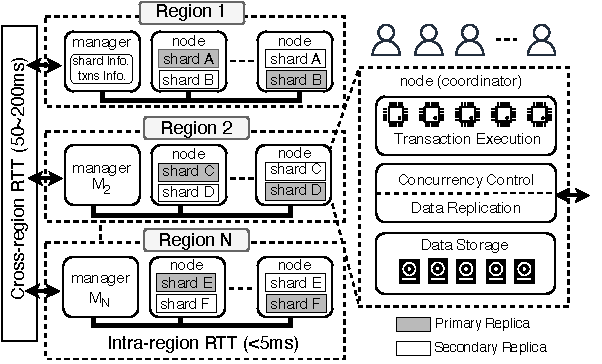
\includegraphics[width=\columnwidth]{figures/deployment.pdf}
\vspace{-10pt}
  \caption{This diagram presents a typical deployment for multi-region databases. The database is partitioned into multiple data shards spanning over multiple regions. Each shard includes a primary replica and several secondary replicas. Intra-region communications are much faster than inter-region communications.}\label{fig:intro}
  \vspace{-10pt}
\end{figure}

In reality, existing consistency models tend to be either overly strong or can be further enhanced without performance degradation. Aggressive models (e.g., strict serializability model ~\cite{papadimitriou1979serializability}) abstract the entire system as a single node, necessitating heavy synchronizations between all computing servers. This approach leads to poor performance in multi-region deployments. Moreover, this model fails to preserve the advantages of near-client computing: even a local transaction has to be ordered with cross-region ones, which is at odds with the motivation of multi-region deployment. Other models provide weaker consistency (e.g., strong snapshot isolation~\cite{daudjee2006lazy}). While these models may suffice for certain application scenarios, the consistency guarantees for local transactions can be further enhanced without much performance overhead: the communication cost for coordinating local transactions can be cheap when using modern hardware and networks. 

% These models use uniform standards for all types of transactions


% (P.3 Many new serializable databases have been proposed, but
% they lack a unified consistency level.)

In this paper, we propose region-linearizable serializability (for short, RLS), the first consistency model to provide as strong as possible consistency for multi-region databases. RLS treats CRTs and IRTs differently. It ensures strict serializability (i.e., the strongest consistency guarantee) for IRTs from the same region and provides regular serializability for CRTs. Specifically, RLS ensures serializability and ``no stale reads'' property (a.k.a. regularity) for all transactions (i.e., both CRTs and IRTs) while preserving real-time order only for the transactions that at least access one same region. For a formal definition, we refer readers to \chref{sec:model}.



To demonstrate the efficiency and applicability of RLS, instead of creating a new transaction protocol from scratch, we design, implement, and evaluate variations of two database systems: Spanner and CockroachDB (for short, CRDB). We refer to these variants as Spanner-RLS and CRDB-RLS, respectively. We chose these two database systems because they complement each other in both the consistency model (strict serializability versus single-key linearizability) and the design of concurrency control protocols (two-phase locking versus timestamp ordering). These two proof-of-concept prototypes pave the way for efficient and practical optimization of distributed protocols when deployed across multiple regions based on a correct-by-construction approach.

Specifically, Spanner and Spanner-RLS follow the design of traditional pessimistic concurrency control: it orders transactions using locks and commits transactions using the two-phase commit. Our variation (Spanner-RLS) significantly reduces CRTs' contention footprint (i.e., locking duration), thus allowing more parallel concurrency. As a result, Spanner-RLS attains $1.16\times$ to $89.01\times$ higher throughput than Spanner while having similar latency.

We present CRDB-RLS as a practical example to demonstrate that databases using weaker consistency models can also benefit from RLS by tightening their consistency guarantees. 
The original consistency model (i.e., single-key serializability) used by CRDB is considerably weaker than RLS.
We implemented regional semantics into CRDB's conflict detection protocol, requiring all conflicting IRTs to be ordered within the regions, even if they access different keys. Given that intra-region communication is significantly cheaper than cross-region communications, the performance overhead of CRDB-RLS can be ignored (e.g., less than $\sim15\%$ in our evaluation). Conversely, the stronger guarantee efficiently eliminates anomalies caused by violating the real-time order, thus simplifying application development~\cite{spanner:osdi12, lu2023ncc}.

\vspace{3pt}
\noindent\textbf{Contributions.} In summary, this paper's contributions stem from a fundamental insight that existing consistency models are inadequately designed for multi-region deployment. To our knowledge, this paper provides the first tailored consistency model for multi-region transactional processing. Our contributions are four-fold: 

\vspace{3pt}
\begin{itemize}[leftmargin=*, itemsep=3pt]
\setlength{\parsep}{0pt}
\setlength{\parskip}{0pt}
\setlength{\parindent}{1em}
  \item We systematically analyze the multi-region deployment model and highlight the limitations of existing consistency models.
  \item We implemented two distinct system variations, Spanner-RLS and CRDB-RLS, to demonstrate the efficiency and applicability of our novel consistency model (RLS). Both of the two prototypes are built on open-source codebases, and the source code is available at {\color{darkred}{\url{https://github.com/vldb24p771/spanner_rls}}} and {\color{darkred}{\url{https://github.com/vldb24p771/crdb_rls}}}, respectively.
  \item We extensively evaluate these variations and present compelling results showcasing the substantial performance improvements achieved by RLS. Specifically, RLS enhances Spanner's performance, achieving throughput improvements ranging from $1.16\times$ to $89.01\times$, and provides more robust consistency guarantees for CRDB without significant performance degradation.
  \item Spanner-RLS and CRDB-RLS can serve as practical templates for the future adoption of RLS to other concurrency control protocols.
% \vspace{1pt}
\end{itemize}
\vspace{6pt}


The rest of the paper is organized as follows. \chref{sec:background} discusses the system model of our multi-region databases deployment, the background of geo-distributed transaction processing, and the motivating applications. \chref{sec:model} details our new consistency model: RLS. \chref{sec:spanner} illustrates the application of RLS to Spanner.  \chref{sec:crdb} delves into CRDB and CRDB-RLS. Finally, a discussion of related works is presented in  \chref{sec:related}, and  \chref{sec:conclusion} concludes the paper.
